\section{Evaluation}
\label{sec:eval}

\subsection{402Pilot-Bench setup}
\label{sec:eval-setup}

\paragraph{Pre-generated dataset.}
We construct \emph{402Pilot-Bench}, a replay-based benchmark in which all LLM responses are pre-generated and frozen. The dataset comprises $823$ tasks across three domains---coding (HumanEval; pass@1), multi-hop QA (HotpotQA; max EM/F1 against gold), and web search (TriviaQA closed-form, plus a custom open-ended subset; LLM-as-judge with a structured rubric). The web-search domain is split into two evaluation buckets because closed-form and open-ended sub-tasks use different evaluators (deterministic max EM/F1 vs.\ cached LLM-as-judge), yielding the four-bucket context partition (T1/T2/T3a/T3b) that PA-DCT uses for contextual bucketing ($K_b = 4$). For each (task, provider) pair we pre-generate $V = 5$ response versions, yielding $823 \times 5 \times 5 = 20{,}575$ total responses scored once at pre-generation time and replayed deterministically across all bandit experiments. Pre-generation decouples bandit evaluation from inference noise and enables exact reproduction of any seed; non-stationarity is introduced by scenario-level transformations of realized failures and effective prices, while the underlying response pool stays fixed for controlled comparison.

\paragraph{Providers.}
Five heterogeneous provider pipelines, deliberately calibrated to expose the same-tier-different-quality phenomenon central to the regime rather than to model a representative market distribution. Table~\ref{tab:providers} summarizes the configuration; the key design point is that P-mid, P-adv, and P-flaky share both base price (\$0.002/call) and base model, so no static rule can distinguish them---only reward feedback can.

\begin{table}[t]
\centering
\caption{Provider set in 402Pilot-Bench. P-mid, P-adv, and P-flaky share the same nominal price tier and base model; only reward feedback distinguishes them. Model names match \texttt{experiments/main.yaml} in the released artifact.}
\label{tab:providers}
\small
\begin{tabularx}{\textwidth}{@{}llXcX@{}}
\toprule
Provider   & Model         & Tools / behaviour              & Price (\$/call) & Notes \\
\midrule
P-cheap    & qwen3.5-flash & none, parametric memory only   & $0.0005$ & weakest, cheapest \\
P-mid      & GPT-5.4-mini  & BM25 retrieval                 & $0.002$  & reliable mid tier \\
P-premium  & GPT-5.4       & CoT + tool use                 & $0.01$   & strongest, priciest \\
P-adv      & GPT-5.4-mini  & adversarial system prompt      & $0.002$  & fluent but wrong \\
P-flaky    & GPT-5.4-mini  & 40\% timeout injection         & $0.002$  & unreliable mid \\
\bottomrule
\end{tabularx}
\end{table}

\paragraph{Task domains and evaluation buckets.}
Tasks come from three domains (coding, multi-hop QA, web search) but are split into four evaluation buckets because the web-search domain uses two different evaluators (deterministic max EM/F1 for closed-form vs.\ LLM-as-judge for open-ended). The four buckets are: T1 coding (HumanEval pass@1, deterministic), T2 multi-hop QA (HotpotQA max EM/F1, deterministic given gold), T3a web-search closed-form (TriviaQA-web, deterministic max EM/F1), T3b web-search open-ended (custom, LLM-as-judge against a fixed rubric, cached at pre-generation). PA-DCT's contextual bucketing operates at the granularity of these four buckets ($K_b = 4$).

\paragraph{Scenarios.}
Three calibrated market scenarios:
\begin{itemize}
\item \emph{S1 --- Stationary.} No mid-run changes; provider behaviour is drawn iid throughout the run.
\item \emph{S2 --- Mid outage.} \texttt{MidOutageScenario(outage\_start=3000, outage\_end=5500, outage\_failure\_rate=0.30)}. Within the $2{,}500$-round outage window, P-mid fails $30\%$ of calls; outside the window, P-mid behaves nominally.
\item \emph{S3 --- Premium promotion.} \texttt{PremiumDropScenario(shock\_round=1000, price\_multiplier=0.2)}. At round $1{,}000$ the effective price of P-premium drops from \$0.01 to \$0.002 (matching the mid tier). The agent has $9{,}000$ post-shock rounds to detect the change and migrate spend.
\end{itemize}

\paragraph{Scale.}
Each (policy, scenario) cell runs $N = 30$ seeds for $T = 10{,}000$ rounds with budget $B = \$50$. At the listed premium price, this budget supports $5{,}000$ premium calls, so S1/S2 expose wallet pressure directly; S3 tests whether a policy can use the lower realized post-shock price rather than continuing to treat P-premium as unaffordable. Within each scenario, policies are evaluated on identical seed paths and the same frozen response set, so paired differences are driven by policy behaviour under the same replay stream.

\subsection{Comparators and metrics}
\label{sec:eval-comparators}

\paragraph{Comparators.}
We compare PA-DCT against five non-oracle baselines and one offline oracle reference, all evaluated on identical seeds:
\begin{itemize}
\item \textbf{Random.} Uniform draw from the affordable set each round.
\item \textbf{Always-P-cheap / Always-P-mid / Always-P-premium.} Three fixed-arm policies covering the price tiers; Always-P-premium is the strongest non-adaptive baseline on quality alone.
\item \textbf{BudgetRule.} A threshold heuristic over remaining wallet fraction---prefer P-premium while the wallet is ample, downgrade to P-mid or P-cheap as the wallet thins. Instantiates a FrugalGPT-style fixed escalation rule~\citep{chen2023frugalgpt}.
\item \textbf{PA-DCT.} Ours.
\item \textbf{True Oracle (upper bound).} A free-running policy that, each round, peeks at every affordable arm's actual outcome at the round's realized response version and picks the one with the highest payment-aware reward at the wallet's current $\lambda_t$. The Oracle owns its own wallet and so its own $\lambda$ trajectory; it is a replay upper-bound reference, not an admissible online policy, because it observes counterfactual outcomes that online policies cannot observe.
\end{itemize}

\paragraph{Metrics.}
Five metrics, locked in advance:
\begin{itemize}
\item \emph{Cumulative payment-aware reward (cum-PA).} $R^\pi_T = \sum_t r_t$, the primary objective the policy optimizes; all paired-bootstrap significance tests are computed on cum-PA.
\item \emph{Mean quality ($\bar q$).} Mean per-round quality $\bar q = (1/T)\sum_t q_t$, a proxy for task-level success at the granularity of the per-task evaluator.
\item \emph{ROI.} $\sum_t q_t / \sum_t c_t$, the quality yield per dollar (a high-ROI policy can spend very little, so it must be read alongside $\bar q$).
\item \emph{Cumulative regret.} $R^{\mathrm{Oracle}}_T - R^{\pi}_T$, the gap to True Oracle on cum-PA.
\item \emph{Adaptation time (AdaptT).} A trailing-$200$-round ROI timing metric for shock scenarios. In S2, it is the rounds after outage onset until ROI returns to at least $95\%$ of the pre-outage level. In S3, where the shock is an opportunity rather than a degradation, it is the rounds until ROI reaches at least $110\%$ of the pre-promotion level; the minimum measurable value is $200$ rounds because of the trailing window. It is undefined in S1.
\end{itemize}

\subsection{Main results}
\label{sec:eval-main}

Table~\ref{tab:main} reports a scenario-relevant subset of the five locked metrics across S1/S2/S3, as means over $30$ seeds. Each scenario shows cum-PA, ROI, and $\bar q$, plus one additional axis: Regret in S1 (where AdaptT is undefined because no shock occurs) and AdaptT in S2/S3 (where shock response is the focal behavior). Regret in S2/S3 is recoverable from the True Oracle cum-PA row minus each policy's cum-PA. Significance markers come from paired-bootstrap two-sided tests of PA-DCT against each baseline on cumulative payment-aware reward (cum-PA), with $p<10^{-3}$ unless noted as \texttt{ns}.

\begin{table}[t]
\centering
\small
\setlength{\tabcolsep}{3.5pt}
\caption{Main results on 402Pilot-Bench, mean over $30$ seeds. cum-PA is reported with paired-bootstrap two-sided significance vs PA-DCT in superscript ($^{\ast\ast\ast\ast}$ $p<10^{-4}$; $^{\textrm{ns}}$ not significant). Bold marks the PA-DCT row, not per-column maxima. ROI = $\sum q_t/\sum c_t$, $\bar q$ is mean quality, Regret is cum-PA gap to True Oracle, and AdaptT is the trailing-$200$ shock-response timing metric defined in \S\ref{sec:eval-comparators}. AdaptT is marked $-$ for non-adaptive baselines (Random, Always-X, BudgetRule), and for the True Oracle row, which observes round-$t$ counterfactual outcomes and so does not undergo online recovery. True Oracle's $\bar q$ and ROI are reported on its own wallet trajectory.}
\label{tab:main}
\resizebox{\textwidth}{!}{%
\begin{tabular}{l|cccc|cccc|cccc}
\toprule
& \multicolumn{4}{c|}{S1 Stationary} & \multicolumn{4}{c|}{S2 Mid Outage} & \multicolumn{4}{c}{S3 Premium Promo} \\
Policy & cum-PA & ROI & $\bar q$ & Regret & cum-PA & ROI & $\bar q$ & AdaptT & cum-PA & ROI & $\bar q$ & AdaptT \\
\midrule
Random            & $3191^{\ast\ast\ast\ast}$ & $209$  & $0.688$ & $3646$  & $3060^{\ast\ast\ast\ast}$ & $205$  & $0.676$ & $-$ & $4382^{\ast\ast\ast\ast}$ & $370$  & $0.688$ & $-$ \\
Always-P-cheap    & $5165^{\ast\ast\ast\ast}$ & $1221$ & $0.610$ & $1672$  & $5164^{\textrm{ns}}$       & $1221$ & $0.610$ & $-$ & $5165^{\ast\ast\ast\ast}$ & $1221$ & $0.610$ & $-$ \\
Always-P-mid      & $5831^{\ast\ast\ast\ast}$ & $410$  & $0.819$ & $1006$  & $5068^{\ast\ast\ast\ast}$ & $379$  & $0.757$ & $-$ & $5831^{\ast\ast\ast\ast}$ & $410$  & $0.819$ & $-$ \\
Always-P-premium  & $-3887^{\ast\ast\ast\ast}$& $87$   & $0.866$ & $10724$ & $-3888^{\ast\ast\ast\ast}$& $87$   & $0.866$ & $-$ & $3113^{\ast\ast\ast\ast}$ & $309$  & $0.866$ & $-$ \\
BudgetRule        & $-82^{\ast\ast\ast\ast}$  & $208$  & $0.831$ & $6919$  & $-408^{\ast\ast\ast\ast}$ & $193$  & $0.769$ & $-$ & $3065^{\ast\ast\ast\ast}$ & $307$  & $0.859$ & $-$ \\
\midrule
\textbf{PA-DCT (ours)} & $\mathbf{5512}$ & $\mathbf{378}$ & $\mathbf{0.797}$ & $\mathbf{1325}$ & $\mathbf{5147}$ & $\mathbf{357}$ & $\mathbf{0.761}$ & $\mathbf{1467}$ & $\mathbf{5911}$ & $\mathbf{429}$ & $\mathbf{0.831}$ & $\mathbf{200}$ \\
True Oracle (UB)  & $6837$ & $561$ & $0.901$ & $0$ & $6809$ & $551$ & $0.901$ & $-$ & $7117$ & $722$ & $0.906$ & $-$ \\
\bottomrule
\end{tabular}%
}
\end{table}

\begin{figure}[t]
\centering
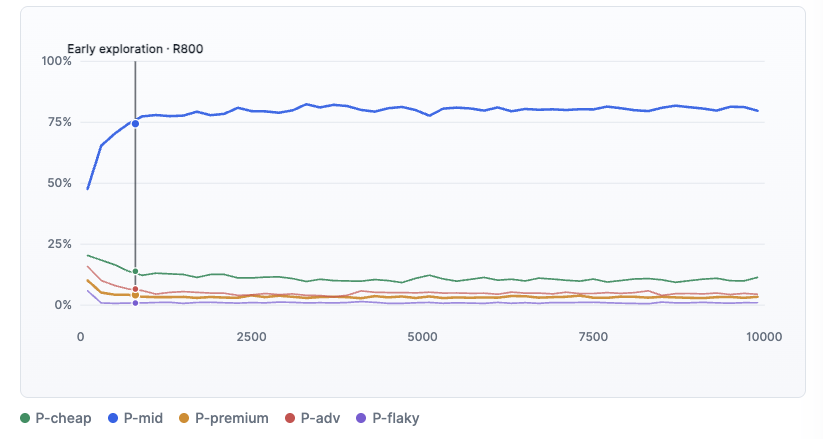
\includegraphics[width=0.32\textwidth]{figures/S1.png}\hfill
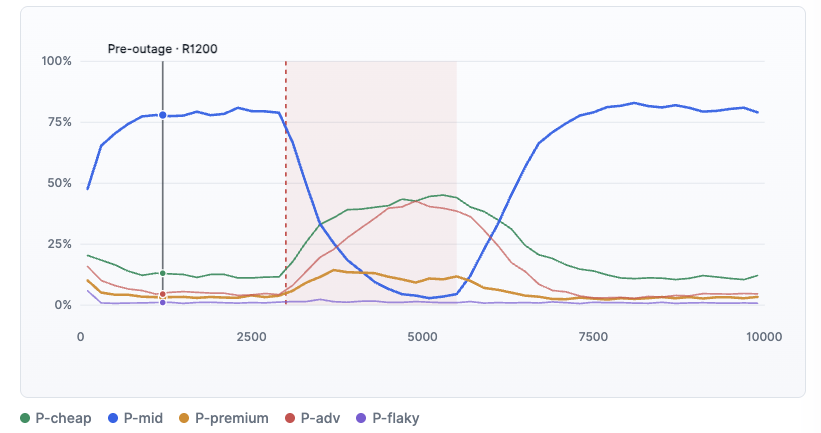
\includegraphics[width=0.32\textwidth]{figures/S2.png}\hfill
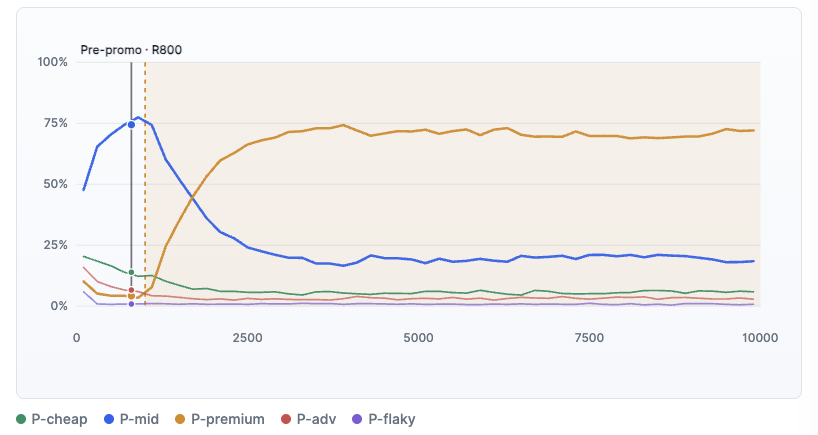
\includegraphics[width=0.32\textwidth]{figures/S3.png}
\caption{PA-DCT provider-allocation share over rounds (mean over $30$ seeds) in S1 stationary (left), S2 mid outage (middle, outage window shaded; window is rounds $3{,}000$--$5{,}500$), and S3 premium promo (right, post-shock region shaded; shock at round $1{,}000$). In S1 the policy converges to a P-mid-dominated mix after the early-exploration phase. In S2 it migrates spend away from P-mid as failures accumulate during the outage and migrates back once P-mid recovers. In S3 it shifts the bulk of spend to P-premium within a few hundred rounds of the price drop. Allocation to P-flaky remains low; P-adv is discussed separately because its detectability depends on the evaluator bucket.}
\label{fig:learning-curves}
\end{figure}

% Figure: trailing-200 ROI around the S2 outage window for full PA-DCT vs the
% $-D$ ablation (the data is reported numerically in Table~\ref{tab:ablations}).
% Adding a dedicated panel is deferred to the camera-ready version; in the
% submission the numerical AdaptT contrast (1467 vs 2249, a 35\% gap) and the
% per-component analysis below already isolate the discount's contribution.

\paragraph{Headline.}
Table~\ref{tab:main} should be read as an adaptation trade-off, not as a claim that PA-DCT is the stationary best arm. S1 is a cost-of-adaptation sanity check: the reliable fixed mid-tier arm is strongest on cum-PA ($5831$), and PA-DCT trails it by $\approx\!319$ because it still explores and maintains shock-readiness in a market with no drift. In the two non-stationary scenarios, PA-DCT outperforms $4/5$ non-oracle baselines in S2 and $5/5$ in S3 on cum-PA; the remaining S2 comparison against Always-P-cheap is a statistically non-significant tie ($5147$ vs $5164$), while PA-DCT delivers much higher mean quality ($0.761$ vs $0.610$). In S3, the learned cost posterior lets PA-DCT capture the premium price promotion, beating Always-P-mid on cum-PA ($5911$ vs $5831$), ROI ($429$ vs $410$), and mean quality ($0.831$ vs $0.819$), while shifting most post-shock spend to P-premium in Fig.~\ref{fig:learning-curves}.

\paragraph{Per-baseline narrative.}
\textbf{vs Random and Always-P-cheap.} PA-DCT dominates Random on cum-PA and mean quality in all scenarios. Against Always-P-cheap, the trade-off is sharper: the cheap arm posts the highest ROI ($\approx\!1{,}221$) by spending very little, but at $\bar q = 0.610$ it leaves quality on the table. PA-DCT wins on cum-PA in S1/S3 and statistically ties in S2, where the cheap arm sidesteps the P-mid outage by never using P-mid; PA-DCT's value in that tied cell is quality, not raw reward.
\textbf{vs Always-P-mid.} Always-P-mid is the stationary fixed-arm benchmark. PA-DCT loses to it in S1, which exposes the exploration cost of a shock-ready policy. Under the S2 outage, Always-P-mid is directly penalized by the $30\%$ failure rate, whereas PA-DCT migrates spend away from P-mid and wins on cum-PA. Under the S3 promotion, PA-DCT uses realized cost feedback to exploit the newly cheap premium arm and improves over Always-P-mid on all three reported economic axes.
\textbf{vs Always-P-premium.} Always-P-premium has the highest fixed-arm mean quality, but in S1/S2 it exhausts the \$50 wallet near round $5{,}000$ and accumulates large negative payment-aware reward under high wallet pressure. In S3 it no longer bankrupts after the price cut, but the first $1{,}000$ expensive premium calls still leave it far behind PA-DCT on cum-PA and ROI.
\textbf{vs BudgetRule.} BudgetRule's static escalation triggers at fixed wallet thresholds and cannot detect the S3 price promotion. PA-DCT migrates to P-premium at the first measurable AdaptT window after the round-$1{,}000$ shock and accumulates substantially more cum-PA over the remaining $9{,}000$ rounds.

\paragraph{Adversarial-provider detection.}
The same-price provider design exposes evaluator-bounded adversarial detection. PA-DCT suppresses P-flaky quickly because timeout feedback is explicit. P-adv is harder: deterministic buckets such as T1/T2 make its low utility visible earlier, while T3b open-ended judging occasionally accepts fluent-but-wrong answers, slowing avoidance. During the S2 outage, some residual P-adv selection also reflects the policy's search for alternatives to degraded P-mid; we revisit this evaluator limit in \S\ref{sec:discuss}.

\subsection{Ablations: which classical components transfer}
\label{sec:eval-ablations}

We disable each of PA-DCT's four conceptual components in turn---Payment-aware ranking ($-P$), Discount ($-D$), Contextual bucketing ($-C$), Thompson sampling ($-TS$). Full PA-DCT is a robust shock-adaptive design, not a per-scenario tuning of the highest cum-PA mean, so the ablation asks which component is exposed on which metric. We additionally run a diagnostic ablation that isolates the cost-posterior pathway inside payment-awareness ($-C_{\mathrm{post}}$, which pins cost to the spec scalar $\bar c_a$ while leaving wallet-pressure weighting intact). This diagnostic is meaningful only under price drift, so we run it on S3 only. Table~\ref{tab:ablations} reports deltas relative to full PA-DCT.

\begin{table}[t]
\centering
\small
\setlength{\tabcolsep}{3.5pt}
\caption{Component ablation: rows $-P,-D,-C,-TS$ ablate the four conceptual components of PA-DCT; row $-C_{\mathrm{post}}$ is a diagnostic isolation of the cost-posterior pathway inside $P$ (it pins cost to the spec scalar $\bar c_a$ while leaving wallet-pressure weighting intact). cum-PA is reported as mean$\pm$std over $30$ seeds; ROI, $\bar q$, Regret, and AdaptT as means. Bold marks the metric that most clearly exposes each component's empirical role; AdaptT is defined in \S\ref{sec:eval-comparators}. The $-C_{\mathrm{post}}$ ablation is run on S3 only because realized prices match $\bar c_a$ in S1/S2; those cells are marked \texttt{n.r.} (not run) rather than inferred.}
\label{tab:ablations}
\resizebox{\textwidth}{!}{%
\begin{tabular}{l|cccc|cccc|cccc}
\toprule
& \multicolumn{4}{c|}{S1 Stationary} & \multicolumn{4}{c|}{S2 Mid Outage} & \multicolumn{4}{c}{S3 Premium Promo} \\
Variant & cum-PA & ROI & $\bar q$ & Regret & cum-PA & ROI & $\bar q$ & AdaptT & cum-PA & ROI & $\bar q$ & AdaptT \\
\midrule
Full PA-DCT      & $5512\pm 54$  & $378$ & $0.797$ & $1325$ & $5147\pm 80$  & $357$ & $0.761$ & $\mathbf{1467}$ & $5911\pm 51$  & $429$ & $\mathbf{0.831}$ & $\mathbf{200}$  \\
$-P$             & $\mathbf{-1710\pm 588}$ & $111$ & $0.839$ & $8547$ & $\mathbf{-1966\pm 507}$ & $103$ & $0.839$ & $1611$ & $4528\pm 369$ & $351$ & $0.840$ & $200$  \\
$-D$             & $5745\pm 95$  & $412$ & $0.810$ & $1092$ & $5113\pm 125$ & $399$ & $0.745$ & $\mathbf{2249}$ & $5974\pm 93$  & $426$ & $0.838$ & $\mathbf{279}$  \\
$-C$             & $5679\pm 41$  & $390$ & $0.812$ & $1159$ & $5225\pm 66$  & $368$ & $0.761$ & $1176$ & $6024\pm 35$  & $425$ & $0.848$ & $\mathbf{398}$  \\
$-TS$            & $5540\pm \mathbf{458}$ & $535$ & $0.740$ & $1297$ & $5063\pm \mathbf{481}$ & $537$ & $0.687$ & $1125$ & $5663\pm \mathbf{244}$ & $552$ & $0.742$ & $\mathbf{2232}$ \\
$-C_{\mathrm{post}}$ & \texttt{n.r.} & \texttt{n.r.} & \texttt{n.r.} & \texttt{n.r.} & \texttt{n.r.} & \texttt{n.r.} & \texttt{n.r.} & \texttt{n.r.} & $\mathbf{5681\pm 54}$ & $423$ & $\mathbf{0.797}$ & $\infty$ \\
\bottomrule
\end{tabular}%
}
\end{table}

\paragraph{$-P$ (no payment-aware): uniformly costly.}
Removing the budget-pressure weighting forces selection by raw utility, causing the policy to favour high-quality but expensive arms and exhaust the wallet early. Cumulative reward collapses below zero in S1/S2 ($-1{,}710 \pm 588$ and $-1{,}966 \pm 507$) and remains far below full PA-DCT in S3 ($4{,}528 \pm 369$ vs $5{,}911 \pm 51$), where the round-$1{,}000$ price drop partially bails the policy out post-shock. \emph{Conclusion}: payment-awareness is necessary in absolute terms; no other ingredient compensates for ignoring wallet pressure.

\paragraph{$-D$ (no discount, $\gamma=1$): visible on adaptation time.}
With $\gamma = 1$, cumulative reward is not the axis that justifies discounting: $-D$ is slightly higher in S1/S3 and close in S2. Under shocks, however, discounting changes the response speed. In S2, full PA-DCT recovers in $1{,}467$ rounds versus $2{,}249$ for $-D$, a $35\%$ acceleration. In S3 the gap is smaller ($200$ vs $279$ rounds) because the $9{,}000$-round post-shock window is long enough for either variant to converge on the new opportunity. \emph{Conclusion}: discount earns its place specifically on AdaptT; cumulative reward alone would miss this role.

\paragraph{$-C$ (no contextual, $K_b = 1$): scenario-dependent.}
Contextual bucketing is not uniformly beneficial in this benchmark. A single global bucket is faster in S2 ($1{,}176$ vs full $1{,}467$ rounds) because the outage hits all task types uniformly and per-bucket fragmentation slows evidence accumulation. It also attains higher cum-PA means in these finite replay runs. In S3, however, full PA-DCT captures the promotion faster ($200$ vs $398$ rounds) because task-type heterogeneity makes the premium arm especially valuable in hard buckets. \emph{Conclusion}: contextual bucketing is a structural choice for heterogeneous task-provider value, not a free win on every aggregate metric.

\paragraph{$-TS$ (no Thompson sampling, greedy posterior mean): variance and opportunity detection.}
Greedy variants are close to full PA-DCT on S1/S2 cum-PA means but have much higher seed-to-seed standard deviation (full $\approx 50$--$80$; $-TS$ $244$--$481$). In S3 the mean gap is also material ($5{,}663$ vs $5{,}911$), and the greedy variant fails to detect the price shock in $6$ of $30$ seeds (AdaptT $2{,}232$ vs full $200$ among runs that do adapt). \emph{Conclusion}: Thompson sampling makes shock detection routine rather than initialization-dependent; mean cum-PA alone hides the risk.

\paragraph{$-C_{\mathrm{post}}$ (no learned cost posterior, $c$ pinned to $\bar c_a$): isolates the price-shock signal.}
With cost held to the spec scalar, the policy is structurally blind to price drift: the C-posterior never updates, so a price drop cannot show up in the sampled $\hatc{a}{k}$ that feeds the decision rule. We measure this on S3, where P-premium's effective price drops to the mid tier at round $1{,}000$ and the cost-posterior pathway has something to track: $-C_{\mathrm{post}}$ keeps treating P-premium as ten-times-more-expensive than mid for the entire post-shock $9{,}000$-round window, P-premium share never crosses $4\%$ (vs $\approx\!60\%$ for full PA-DCT), $\bar q$ stays at the S1 level $0.797$, and AdaptT is undefined ($\infty$) because the trailing-$200$ ROI never reaches the promotion-capture threshold. The cum-PA gap of $-230$ ($p<10^{-4}$, paired bootstrap, $30$ seeds) is the price-shock-specific value of the dual posterior. We did not run the S1/S2 cells of this ablation: realized prices match $\bar c_a$ throughout in those scenarios, so we expect (but did not measure) coincidence with full PA-DCT---the table's $-C_{\mathrm{post}}$ row marks those cells \texttt{n.r.} rather than inferring values. \emph{Conclusion}: removing the learned cost posterior collapses S3 to the no-shock baseline. The four classical components $(P,D,C,TS)$ together cannot recover this; the cost posterior is the structural commitment that makes price shocks first-class observations rather than configuration metadata.

\paragraph{Why five metrics, not one.}
No single classical bandit metric reveals all of these contributions. Cumulative reward alone misses $-D$'s adaptation-speed role and can make $-C$ look uniformly preferable in this finite benchmark. ROI alone over-rewards $-TS$ (greedy locks onto cheap arms with high $q/\$$ ratio while missing better-quality opportunities). AdaptT without cumulative reward would miss $-P$'s collapse in S1/S2. Mean quality $\bar q$ exposes $-C_{\mathrm{post}}$'s failure to migrate to P-premium under the S3 promo (where it stays at the S1 quality level, $0.797$) even though its cum-PA gap is moderate. Regret to the Oracle isolates the cost of $-P$ in the stationary regime where AdaptT is undefined. The five metrics together expose each component on the axis where it matters; this is the multi-metric evaluation framework we recommend for future work in this regime.
